\documentclass{article}
\usepackage{amsmath}
\usepackage{hyperref,graphicx}
\DeclareMathOperator\erf{erf}
\title{A Rough Guide to CladeAge\\
{\small Setting fossil calibrations in BEAST 2}}
\author{Michael Matschiner \\
Remco Bouckaert\\ 
\url{michaelmatschiner@mac.com}\\
\url{remco@cs.auckland.ac.nz}}

\begin{document}
\maketitle
\begin{center}
\includegraphics[width=0.3\textwidth]{cladeage_256x256px.png}\end{center}
\tableofcontents

\section{Introduction}
CladeAge is a program that can be used for specifying fossil calibrations on phylogenies when an estimate of a fossil sampling rate is available. CladeAge can be run as stand alone program or as BEAST 2 add-on. To run CladeAge as a standalone program, there is a Windows, Mac and Linux version -- there are links on  \url{http://beast2.cs.auckland.ac.nz/index.php/CladeAge} to point to the various versions. Alternatively you can run it from the source code, available from \url{http://code.google.com/p/cladeage}. CladeAge is written in Java.

If this guide still leaves questions you can contact the authors,
or consult the BEAST user list on \url{http://groups.google.com/group/beast-users}.

\subsection{Windows}
Download the zip file linked from
\url{http://beast2.cs.auckland.ac.nz/index.php/CladeAge}.
Unzip the file, and an executable {\tt CladeAge.exe} program
is available. Double click the file to start.

\subsection{Mac}
Download the dmg file linked from
\url{http://beast2.cs.auckland.ac.nz/index.php/CladeAge}.
Open the dmg file, and drag CladeAge to the Application directory,
from where you can start it.
\begin{center}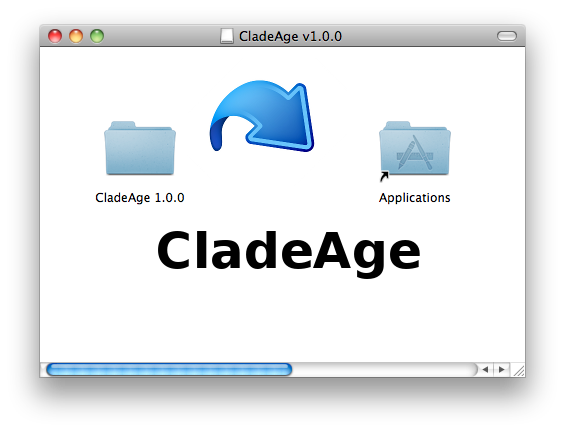
\includegraphics[width=0.5\textwidth]{mac.png}\end{center}

\subsection{Linux}
Download the jar file linked from
\url{http://beast2.cs.auckland.ac.nz/index.php/CladeAge}
and from the command line use

{\tt java -jar cladeage.jar}

to start CladeAge.

\subsection{BEAST}

To use CladeAge in BEAST 2, you need
to install BEAST 2 -- see \url{http://beast2.cs.auckland.ac.nz} for details.
Further, you need the CladeAge add-on. The easiest way to install this
is by running BEAUti, use the menu File/Manage add-ons. 
\begin{center}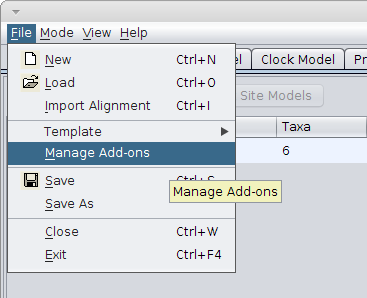
\includegraphics[width=0.3\textwidth]{fileManageAddOns.png}\end{center}
A window pops up
with a list of installed and available add-ons. Click the CladeAge addon, and 
press the Install/Uninstall button.
\begin{center}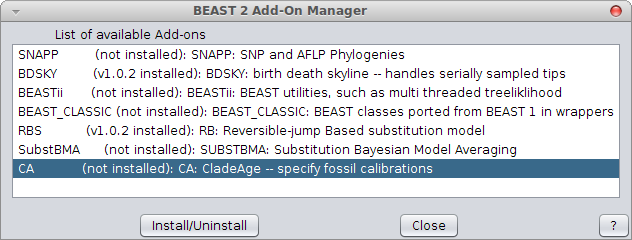
\includegraphics[width=0.7\textwidth]{addonmanager.png}\end{center}

Alternatively, for cluster computers wihtout GUI access, you can use the 
command line utility `addonmanager':

\begin{verbatim}
 Usage: addonmanager [-list] [-add <NAME>] [-del <NAME>] [-useAppDir] [-dir <DIR>] [-help] 
   -list List available add-ons
   -add Install the <NAME> add-on 
   -del Uninstall the <NAME> add-on 
   -useAppDir Use application (system wide) installation directory. Note this requires 
              writing rights to the application directory. If not specified, the user's 
              BEAST directory will be used.
   -dir Install/uninstall add-on in directory <DIR>. This overrides the useAppDir option
   -help Show help
\end{verbatim}
Use 'addonmanager -add CA' to install the CladeAge add-on.

\section{How CladeAge works}

Based on the assumption of a time-constant sampling rate for fossils, CladeAge calculates the probability density $f_t$ for the time of the first occurrence of a clade in the fossil record, $t_f$, given the time of clade origin, $t_o$. As the time of clade origin $t_o$ is unknown prior to the BEAST analysis, CladeAge calculates this probability density $f_t$ for 100 time points older than the clade's first occurrence $t_f$, and draws a probability distribution from the calculated probability densities. These distributions can be used directly as divergence prior distributions in BEAST analyses.

\subsection{The sampling rate}

Probability distributions calculated with CladeAge are based on estimates of the sampling rate of fossils, whereby this rate is assumed to be a time-constant Poisson process. The concept of a sampling rate of fossils is commonly used in the paleontological literature, and is considered to include all processes that lead to the identification and scientific description of a fossil. Thus, the sampling rate encompasses deposition of an organism in the sediment, fossilisation, survival of geological processes, outcropping of the rock formation including the fossil, discovery, correct taxonomic identification, and publication of the fossil find.

Estimates of sampling rates can be obtained by a variety of methods, including the freqRat method of Foote and Raup (1996), the survivorship analysis of Foote (2001), and the analysis of waiting times between sampling events, introduced by Solow and Smith (1997). All these methods have in common that a very large number of fossils, and ideally full occurrence data, i.e. information for each known fossil of a given group, is needed for reliable sampling rate estimates. Thus, for most studies aiming to time-calibrate phylogenies, the estimation of sampling rates for the investigated group is beyond the scope of the analysis. Fortunately however, sampling rates have already been estimated and published for many groups and can readily be used in CladeAge. For example, Foote et al.\ (1999) estimated the sampling rate of Late Cretaceous mammals as 0.03-0.06, Alba et al.\ (2001) found the sampling rate of Iberian mammals of the Neogene to be around 0.8, and Foote and Raup (1996) determined the sampling rate of European Jurassic bivalves to be around 0.41, all values given are per lineage and per million years.

Previously, sampling rates have often been published on genus level instead of species level, and not per million years, but for shorter or longer time bins (Foote \& Raup 1996, Foote \& Sepkoski 1999, Friedman \& Brazeau 2011). In order to use these estimates in CladeAge, they must be transformed into species-level estimates per million years (assuming that fossil ages are also specified in million years in BEAST). One way to transform genus level estimates into species level estimates is to calculate the average number of extant species per genus in the investigated group, assuming that this ratio also holds for fossil members of the same group. If rates have been given for time bins other than a million years, the rate conversion can be performed e.g.\ with the function `sProb2sRate' of David Bapst's R package `paleotree' (Bapst 2012).

\subsection{Clade age probabilities}

If we assume a time-constant sampling rate $\psi$, it can be shown that the probability density $f_t$ for the time of first occurrence of a clade, $t_f$, is

\begin{equation}
f_t = \psi N e^{-\psi S}
\end{equation}
where $S$ is the sum of lineage durations between $t_o$ and $t_f$ (the entire unobserved history of a clade; see Fig. 1), and $N$ is the number of lineages extant at time $t_f$.
\begin{figure}[b!]
\centering
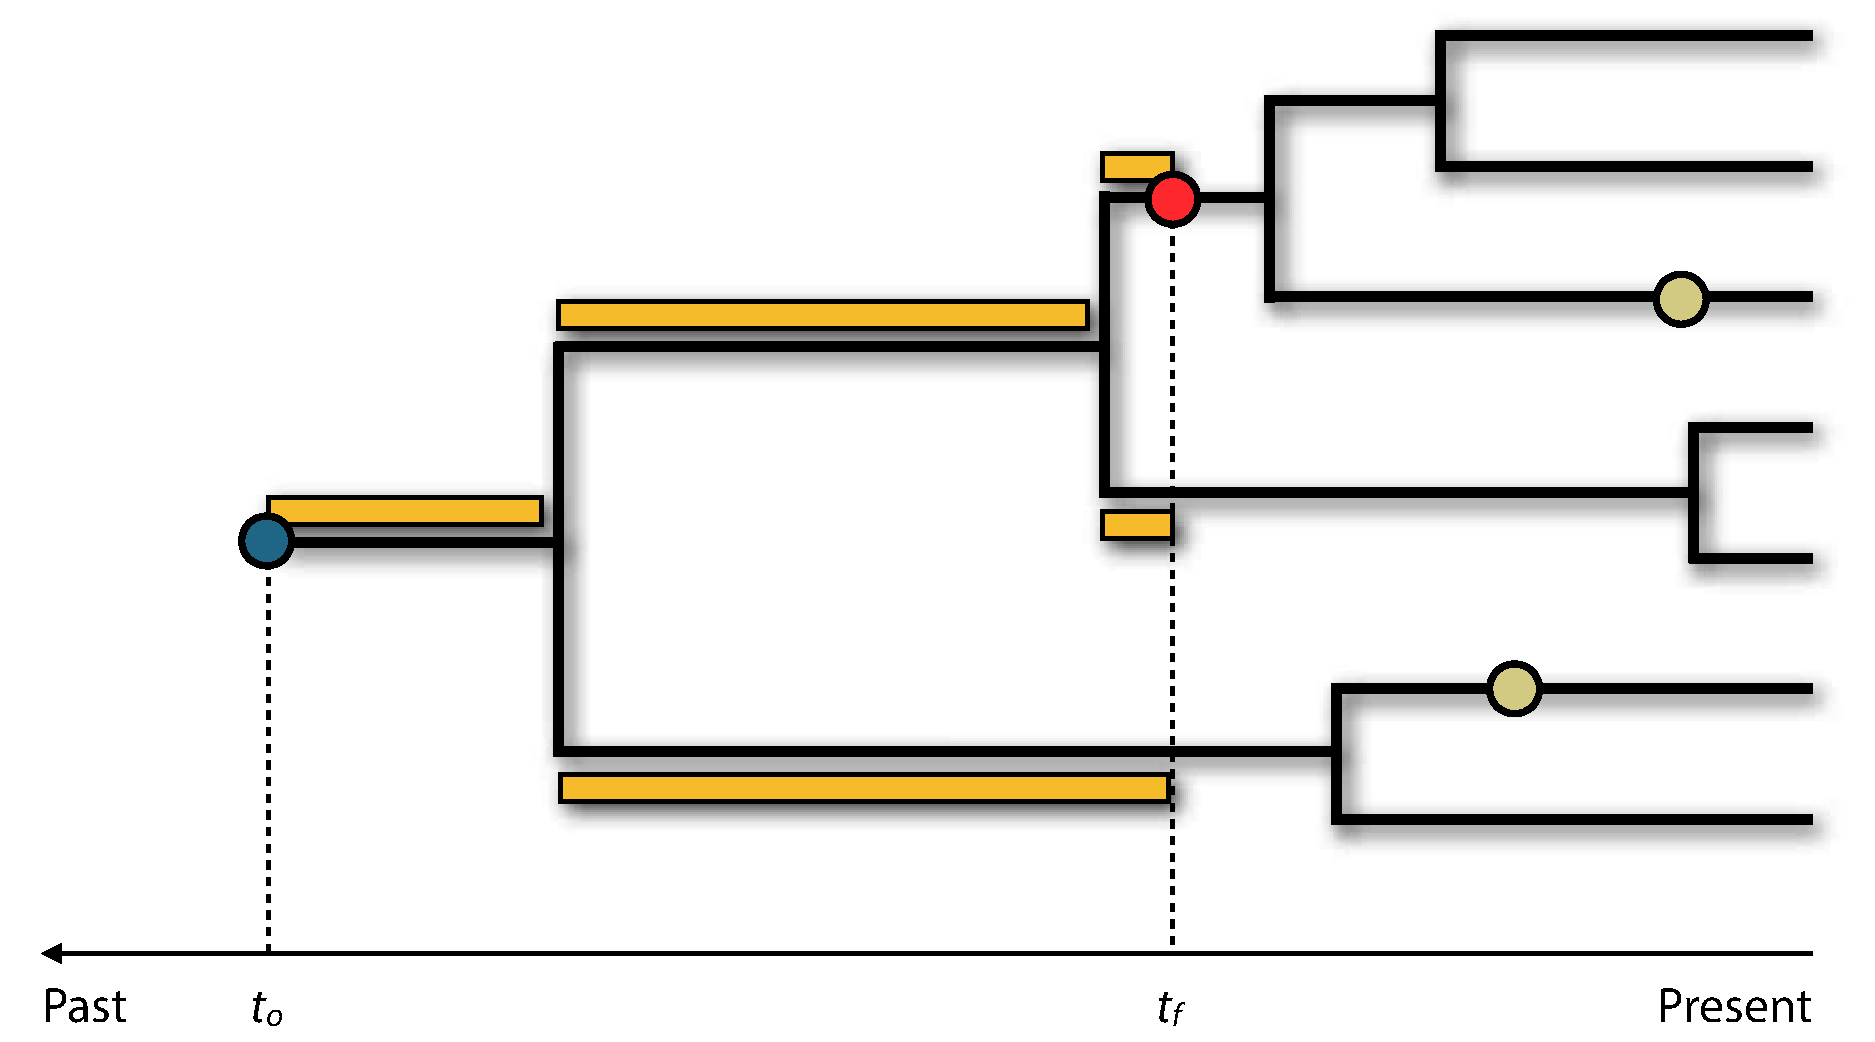
\includegraphics[width=0.99\textwidth]{sumOfLineageDurations}
\caption{Exemplary phylogeny with clade origin at time $t_o$ in blue, the earliest fossil occurrence at time $t_f$ in red and younger fossils in grey. The part of the phylogeny that represents $S$, the sum of lineage durations before the first occurrence, is highlighted in orange.}
\end{figure}

Before running a time-calibration analysis, all we know about $S$ and $N$ is that $S \geq 0$ and $N \geq 1$, as at least one lineage must have existed at the time of the clade's first occurrence. However, we can model the unobserved clade history between $t_o$ and $t_f$ with a birth-death process, assuming time-constant speciation rate $\lambda$ and extinction rate $\mu$. This process must be conditioned on the survival of at least one lineage. As we're now dealing with a conditioned stochastic process, the probability density $f_t$ becomes

\begin{equation}
f_t = \mathrm{E}[\psi N e^{-\psi S} | N \geq 1].
\end{equation}
Unfortunately, we can not solve $f_t$ analytically. Therefore CladeAge generates a large number of birth-death trees with user-specified speciation rate $\lambda$ and extinction rate $\mu$, infers $S$ in each of these trees as the sum of all branch lengths, and calculates $\psi N e^{-\psi S}$ if the birth-death process resulted in $N \geq 1$. According to the law of large numbers, the mean of a large sample converges to its expected value, therefore the probability density $f_t = \mathrm{E}[\psi N e^{-\psi S} | N \geq 1]$ can be calculated as the mean of all these values for $\psi N e^{-\psi S}$. This process is repeated for 100 different tree durations, according to the durations between 100 tested time points for $t_o$ and the fixed value of $t_f$.

\subsection{Probability distributions}

After probability densities have been calculated for 100 time points, CladeAge allows several ways to turn them into probability distributions:

\begin{itemize}
\item
{\bf Empirical CladeAge distribution}: In what we call `\emph{empirical CladeAge distributions}', the calculated probability densities are used directly for the respective time points. Probability densities for times in between these time points are interpolated from the probability densities of the two neighbouring time points, using a linear regression. For all times older than the oldest sampled time point (the tail of the distribution), probability densities are approximated by an exponential distribution that is calculated on the basis of the two oldest time points, so that the probability densities calculated for these two time points lie on this exponential distribution. Finally, \emph{empirical CladeAge distributions} are scaled so that the total probability mass becomes 1. \emph{Empirical CladeAge distributions} are useful when calculation times are allowed to be on the order of seconds, and are the only available distribution type when a sampling gap (see below) is specified. \emph{Empirical CladeAge distributions} are available as divergence priors in BEAST 2 if the CladeAge add-on is used.

\item
{\bf Fitted CladeAge distribution}: CladeAge allows the fitting of what we call `\emph{fitted CladeAge distributions}' to the calculated probability densities. These distributions are similar to truncated lognormal distributions, except that the parameterisation is simplified. The probability density function of an \emph{fitted CladeAge distribution} is as follows:

\begin{equation*}
f_{u} =
\begin{cases}
0, & \mbox{if } u \leq 0 \\
\frac{c}{u + s} \times e^{\frac{-(\mathrm{ln}(u+s) - m)^2}{w}}, & \mbox{if } u > 0,
\end{cases}
\end{equation*}

where $u = t_o - t_f$ and parameters $c$, $s$, $m$, and $w$ (all $\geq 0$) can be optimised so that $f_{u}$ fits the calculated probability densities and its integral sums to 1. We have chosen to introduce this type of distribution, because we found truncated lognormal distributions to provide a near-perfect fit to the calculated probability densities, however the parameterisation of lognormal distributions makes analytical handling unnecessarily complicated. While providing the same fit as truncated lognormal distributions, the simplified parameterisation of \emph{fitted CladeAge distributions} facilitates analytical solution of distribution parameters, as well as analytical integration of the distribution.

Knowing the integral of a distribution is necessary in order to analytically account for uncertainty in the age of first occurrence (see section 2.5). The integral of an \emph{fitted CladeAge distribution} is

\begin{equation*}
\int_0^a \! f_{u} \, \mathrm du=
\begin{cases}
0, & \mbox{if } a \leq 0 \\
-\frac{c \sqrt{\pi w}}{2} \times \erf(\frac{m - \mathrm{ln}(a+s)}{w}), & \mbox{if } a > 0,
\end{cases}
\end{equation*}

where erf is the error function, which CladeAge calculates via a numerical approximation with a maximal error of $1.2 \times 10^{-7}$ (Press et al. 1992).

The analytical solution of the parameters of an \emph{fitted CladeAge distribution} is possible when probability densities of only 4 instead of 100 time points are considered, and the fit of the distribution is only slightly worse if these four time points are carefully selected \emph{a priori}. This massively reduces computation time not only by the limited number of time points for which probability densities must be calculated, but also because the analytical solution of distribution parameters is much faster than the distribution fitting through minimisation of root mean square deviations. As a result, the time needed for the calculation of \emph{fitted CladeAge distribution} parameters is on the order of 0.005 seconds. Of course, if prior distributions are calculated just once before a time-calibration analysis, it hardly matters whether this calculation takes 0.005 s or 1 s. However, the fast analytical calculation of distribution parameters allows repeatedly recalculating these parameters during a BEAST run without substantial delay. In this case, diversification rates $\lambda$ and $\mu$ do not need to be specified by the user. As the BEAST MCMC estimates these parameters anyway, these estimates can be used directly for \emph{fitted CladeAge distributions}. Whenever the BEAST estimates for $\lambda$ and $\mu$ change during the MCMC run, \emph{fitted CladeAge distributions} are recalculated with the updated estimates. %{\bf This is work in progress, and this option is not yet available in BEAST}.

\item
{\bf Standard distributions}: 
Besides \emph{empirical} and \emph{fitted CladeAge distributions}, CladeAge allows the fitting of commonly used distribution types against the calculated probability densities. Available distributions include {\bf exponential}, {\bf lognormal}, {\bf normal} and {\bf gamma distributions}. These distributions are scaled during the fitting process, however the scaling factor is not reported and should be ignored when these distributions are used as priors in Bayesian analyses, otherwise the probability mass of the distribution would not sum to 1.

\if0 TRUNCATED DISTRIBUTIONS ARE NOW DEPRECATED
\item
{\bf Truncated standard distributions}: If the first occurrence age is known without uncertainties (see section 2.5), {\bf truncated lognormal}, {\bf truncated gamma}, and {\bf truncated normal distributions} can be fitted to the calculated probability densities. As with untruncated distributions, these are scaled during the fitting process and the scaling factor is not reported, but unlike untruncated distributions, truncated distributions will not sum to 1 anyway. {\bf This is work in progress, and this option is not yet available in BEAST}.
\fi
\end{itemize}

\subsection{Model parameters}
The model described above requires three parameters: The sampling rate $\psi$ as well as two diversification rates needed for tree simulations, the speciation rate $\lambda$ and the extinction rate $\mu$. However, diversification rates are more easily estimated, and more commonly reported in the literature as net diversification rate $\lambda - \mu$ and turnover rate $\mu / \lambda$. Therefore, CladeAge is written to accept net diversification rate and turnover rate, rather than speciation rate and extinction rate, as input, even though internally, it infers speciation and extinction rates from the specified values for net diversification rate and turnover rate.

\begin{figure}[b!]
\centering
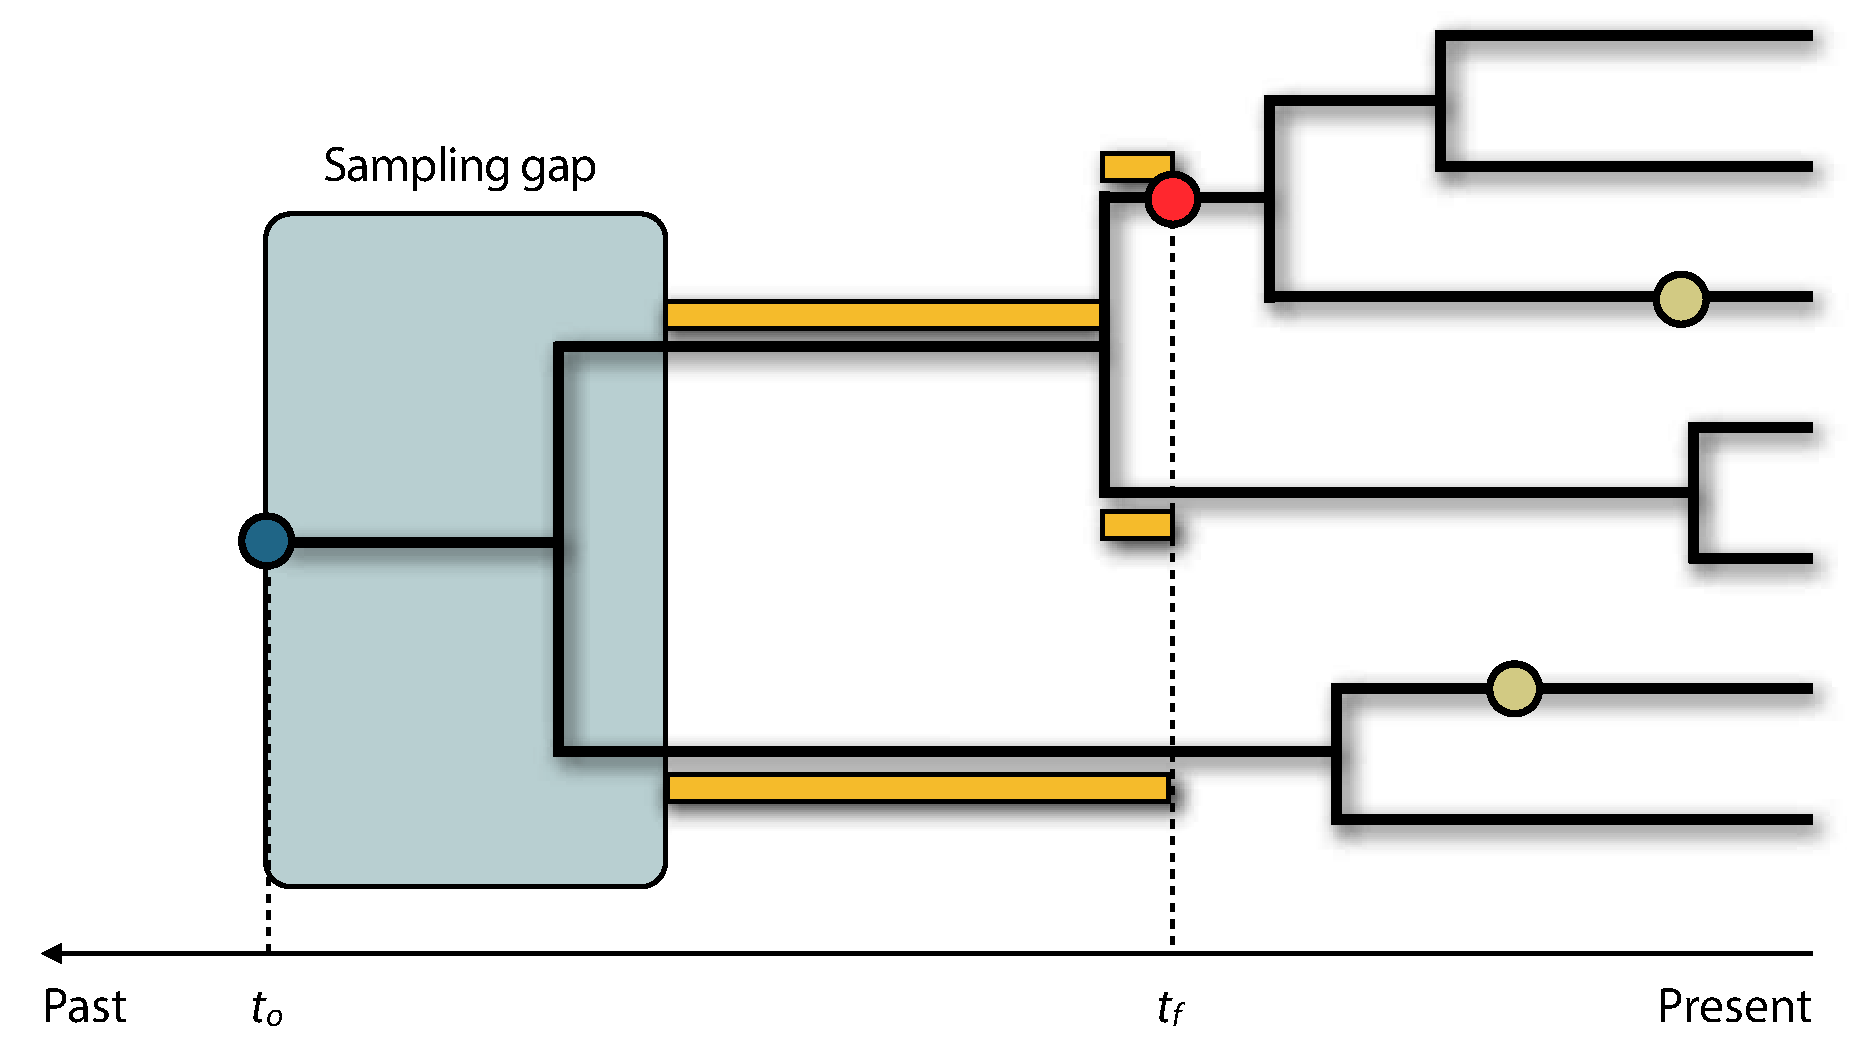
\includegraphics[width=0.99\textwidth]{samplingGap}
\caption{The sampling gap at the beginning of a clade's history represents the time period during which preservation potential is considered negligible. Use of a sampling gap effectively truncates the sum of lineage durations (with preservation potential) $S$ between $t_o$ and $t_f$.}
\end{figure}

For some of the analyses available in CladeAge, a fourth parameter can be specified, the so-called sampling gap. The sampling gap represents the time period at the very beginning of a clade's history, for which we assume that preservation potential has been negligible, which effectively sets the sampling rate $\psi$ to zero for this period. There are several reasons why one might assume the existence of a sampling gap: For example, the populations sizes of a clade might be very small shortly after its origination, which would reduce the potential to become preserved in the fossil record. Similarly, if the population has been geographically limited to a small region, which is more likely at the beginning of a clade's history, this would also lower preservation potential. One might also assume that clades require time to evolve morphological features that allow fossils to be assigned to these clades. As the sampling rate $\psi$ includes all processes from the fossilisation of an organism to its discovery and correct taxonomic assignment, $\psi$ would also be zero for the time before the emergence of recognisable morphological features of a clade.

Whether or not a sampling gap should be used is debatable, as one might argue that over time periods of millions of years, as are usually considered when phylogenies are time-calibrated, the times required to reach substantial population sizes and geographic distributions, or to evolve recognisable morphological features, are negligible. In fact, the latter may even go simultaneously with clade origination according to the theories of punctuated equilibrium and key innovations (Rabosky et al. 2013). If a sampling gap is used, CladeAge truncates the older end of all generated trees by the duration specified as sampling gap before calculating the probability density $f_t$ (see Fig. 2). 

\subsection{Taking parameter uncertainties into account}

In real world data sets, all parameter estimates have uncertainties. In order to account for these uncertainties, CladeAge allows the specification of minimum and maximum values for all parameters. Between these minimum and maximum values, CladeAge always assumes equal probabilities for all values (this is equivalent to uniform hyperpriors on all CladeAge parameters). Internally, the way how these uncertainties are taken into account in CladeAge differs between the parameters, and between the distribution types.

The only uncertainty that is always accounted for in the same way, is that of the sampling rate. This uncertainty is always analytically integrated out when probability densities are calculated.

Uncertainties in the net diversification rate $\lambda - \mu$ and the turnover rate $\mu / \lambda$ are accounted for by randomly drawing values from the specified ranges for each iteration of tree generation and calculation of $f_t$. As a large number of iterations is used (usually 10000 iterations), this is effectively the same as integrating over the range of uncertainty. Only when the calculation time must be minimised (when CladeAge distributions are recalculated during the BEAST MCMC), are the uncertainties of net diversification rate and turnover rate used in a slightly different way. In this case, values for each iteration are not drawn from the range at random. Instead a fix number of values (currently set to 30 values for both rates) is chosen to represent the entire ranges of uncertainties of both the net diversification rate and the turnover rate. A sufficient number of iterations is then used to combine all values for the net diversification rate with all values for the turnover rate. This results in the same probability densities as when values are drawn at random, however fewer iterations are needed to obtain the same accuracy, which serves to speed up the calculations.

For technical reasons, the sampling gap can only be used in combination with \emph{empirical CladeAge distributions}. If a sampling gap is used, and uncertainties in the duration of the sampling gap are specified, these are accounted for by randomly drawing from the range between the minimum and maximum sampling gap for each iteration of tree generation and calculation of $t_f$, in the same way as the uncertainties of net diversification rate and turnover rate are taken into account.

Finally, uncertainties in the time of the first occurrence of a clade are accounted for differently, depending on whether \emph{empirical CladeAge distributions} are used or not. If an \emph{empirical CladeAge distribution} is to be calculated, first occurrence ages are drawn at random from the range between minimum and maximum first occurrence age. \emph{Fitted CladeAge distributions}, however, are calculated only based on the minimum first occurrence age, and are then analytically integrated over the range of uncertainty. For all other types of distributions, probability densities are calculated based on only the minimum first occurrence age, as for \emph{fitted CladeAge distributions}, but are numerically integrated over the range of uncertainty before the distribution is fitted.

\section{CladeAge input}

The following parameters can be used in CladeAge:
\begin{itemize}
\item
{\bf First occurrence age}: The age of the oldest fossil of the clade. If this age is known exactly, it should be specified in the 'Minimum' field. If not, you should specify both a minimum and maximum age. Consider a fossil described in the literature to be Oligocene in age. The Oligocene extends from about 34 million to 23 million years before the present ($33.9\pm 0.1$ to $23.03\pm 0.05$ Ma). The uncertainties in the boundaries are small enough to be ignored, so the minimum is 23.03 and maximum 33.9 if you want to express ages in millions of years. 

\item
	{\bf Net diversification rate}: The net diversification rate is the difference between speciation $\lambda$ and extinction rate $\mu$. 
See e.g. Alfaro et al. (2009), Santini et al. (2009), Jetz et al. (2012), and Stadler (2011) for rate estimates for vertebrates, teleost fishes, birds, and mammals. 

\item
	{\bf Turnover rate}: The turnover rate is the ratio of extinction and speciation rate ($\mu/\lambda$). If no turnover rate is specified, CladeAge assumes it to be zero, which also means that the extinction rate $\mu$ is equal to zero.

\item
	{\bf Sampling rate}: The sampling rate $\psi$ (sometimes called 'preservation rate') includes all processes that result in the publication of a fossil, including fossilization, discovery, identification and description (Friedman \& Brazeau 2011). Estimates have been reported for many taxonomic groups (e.g. Foote et al. 1999, Foote \& Sepkoski 1999) and can be obtained by methods outlined in Foote (1997).

\item
{\bf Sampling gap}: The sampling gap represents the time period after a clade's origin during which it could not have fossilized (possibly due to small population size or limited geographic distribution), or its earliest fossils could not be recognized as part of this clade (as no recognisable morphological features of this clade may have evolved yet). Specifying a sampling gap is optional and it can only be used in combination with empirical probability distributions. A sampling gap of 0.0-2.0 Ma may be a reasonable assumption.
\end{itemize}

\section{Stand alone CladeAge}
When starting CladeAge, something similar to this should show up:
\begin{center}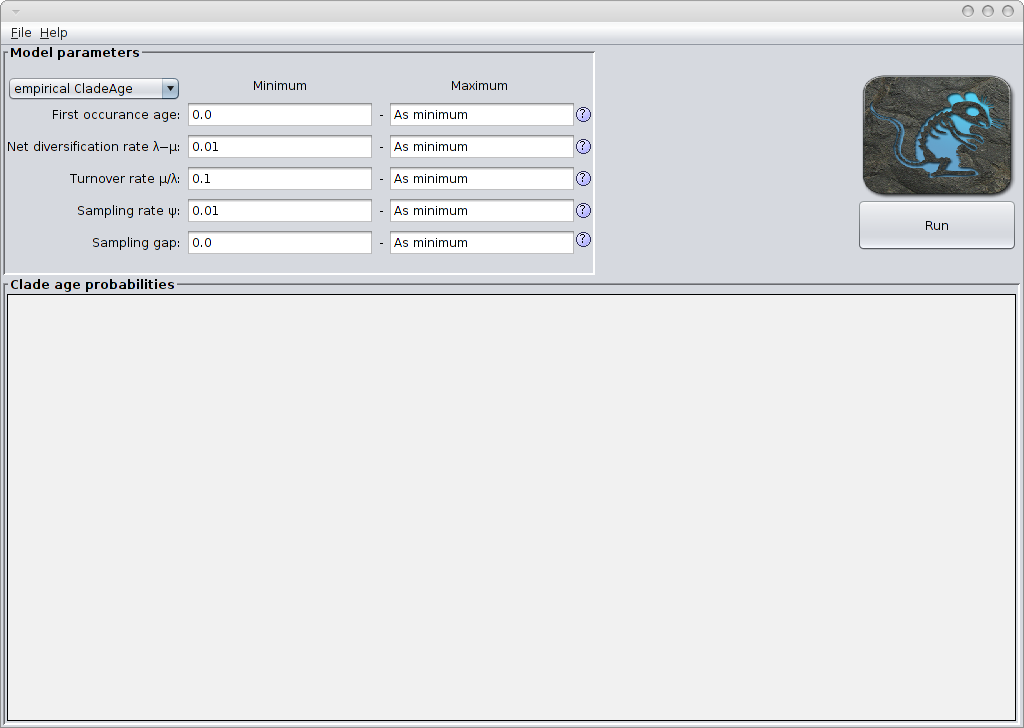
\includegraphics[width=\textwidth,clip=true,trim=0 0 0 0]{ca.png}\end{center}
You can specify the fossil related parameters, and press 'Run' to get a preview
of the distribution.

% THE MODE MENU IS NOW DEPRECATED 
%Select the menu 'Mode' and click 'Show advanced settings' to display the simulation
%related settings and which distribution to fit.
%\begin{center}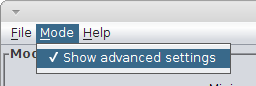
\includegraphics[width=0.4\textwidth,clip=true,trim=0 0 0 0]{menuMode.png}\end{center}

\begin{center}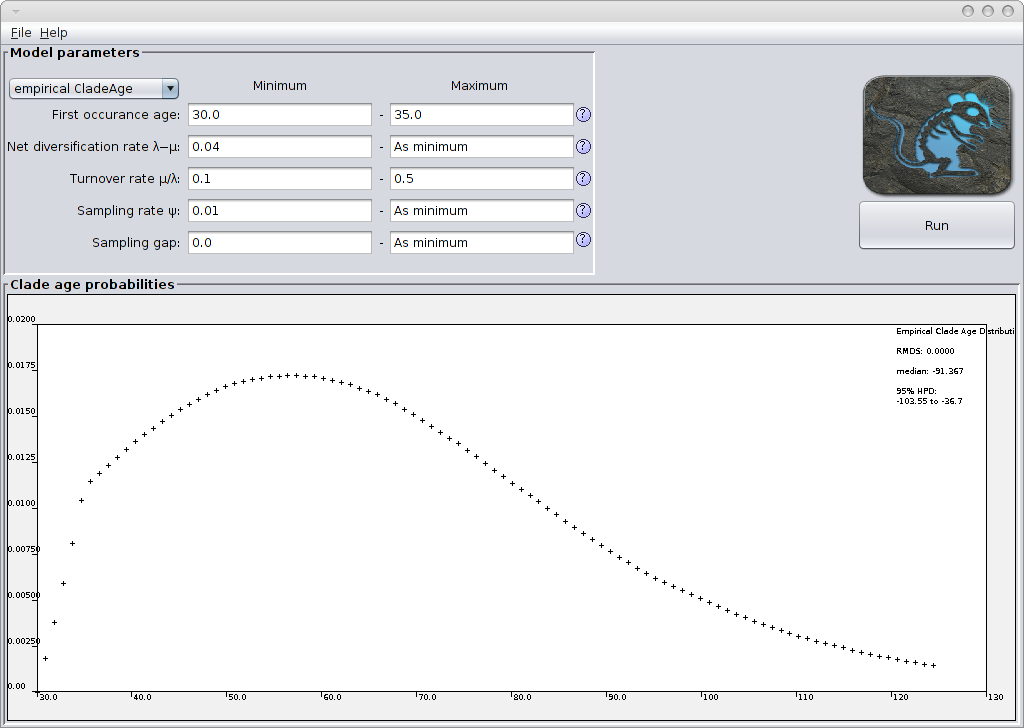
\includegraphics[width=\textwidth,clip=true]{ca2.png}\end{center}
Click the panel with the graph to show statistics, that you can copy on the clipboard.
Likewise, clicking any of the question-mark buttons shows helpful information, 
including citations you can copy.
\begin{center}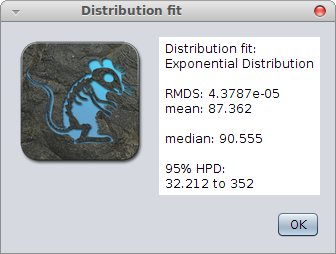
\includegraphics[width=0.35\textwidth]{help.png}\hskip1cm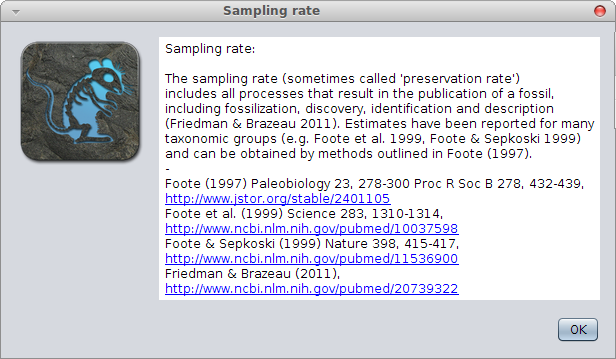
\includegraphics[width=0.55\textwidth]{help2.png}
\end{center}



\section{CladeAge in BEAST}
When CladeAge is installed, a new 'Fossil Priors' tab is added.
\begin{center}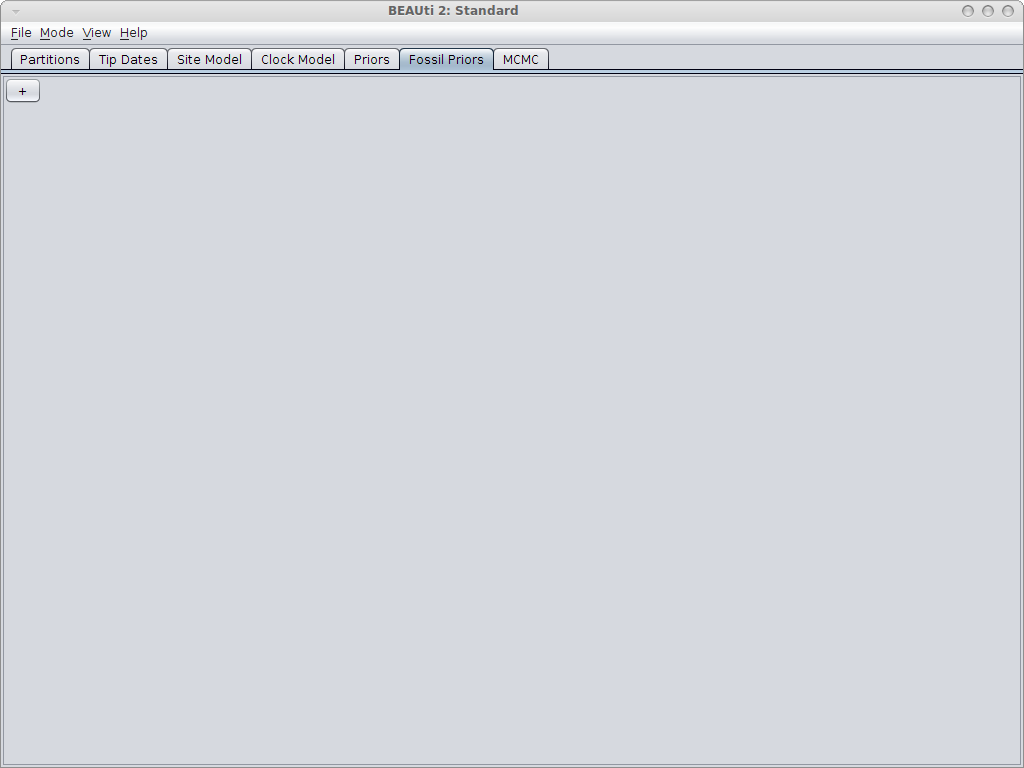
\includegraphics[width=\textwidth,clip=true,trim=0 300 0 0]{fossilPriorsTab.png}\end{center}
To specify a new fossil calibration, click the plus in the Fossil Priors tab, 
and a dialog pops up where you can specify a clade. This clade should contain
taxa where there is morphological evidence that the taxa are descendants of
a common ancestor of the fossil. Enter the name of the clade,here 
human-chimp, and select the taxa you want in your clade.
\begin{center}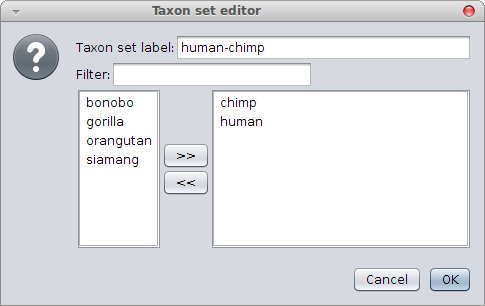
\includegraphics[width=0.7\textwidth]{taxonSetDialog.png}\end{center}
Click the OK button, and now the Fossil Priors tab looks similar to this;
\begin{center}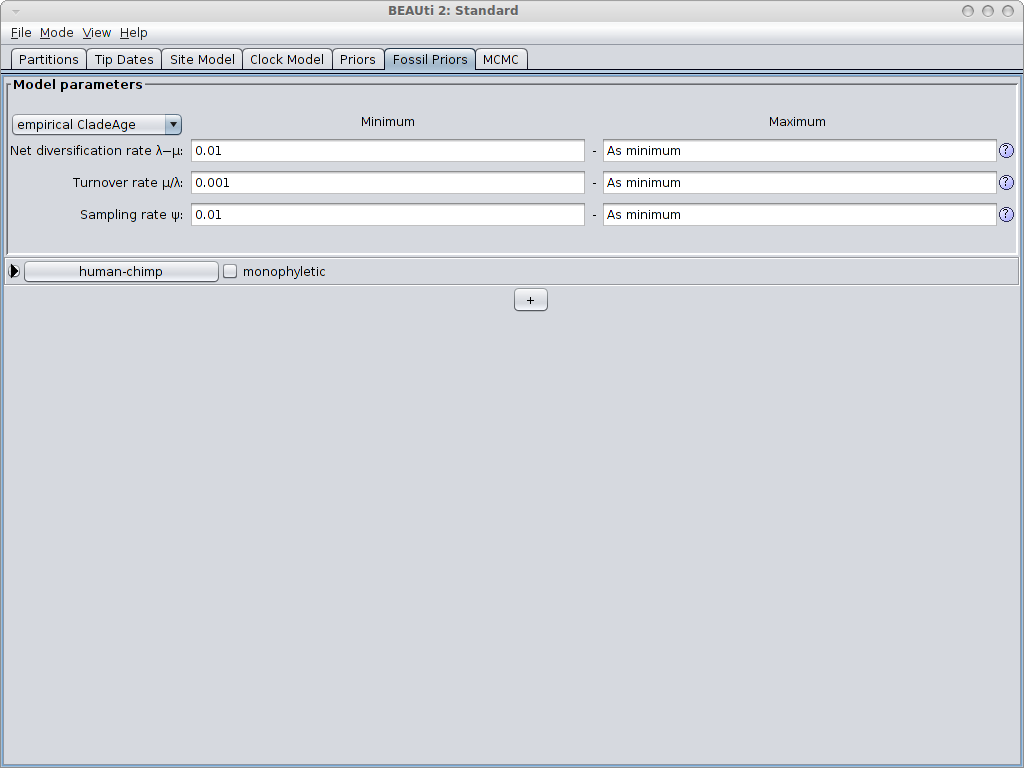
\includegraphics[width=\textwidth,clip=true,trim=0 300 0 0]{fossilPriorsTab2.png}\end{center}
The divergence rate, turnover rate and sampling rate are assumed to be the same
for all calibrations, which is a reasonable assumption for most situations
\footnote{This can be changed by editing the XML. For each variant of divergence
	rate, turnover rate and sampling rate, a new parameter needs to be specified
	and the appropriate {\tt FossilCalibration} should refer to these parameters.}.
The clade can be enforced to be monophyletic by clicking the 'monophyletic' check box
next to the clade name.

To specify the remaining parameters -- fossil occurance age and fossil gap -- click the 
little triangle next to the clade name.
\begin{center}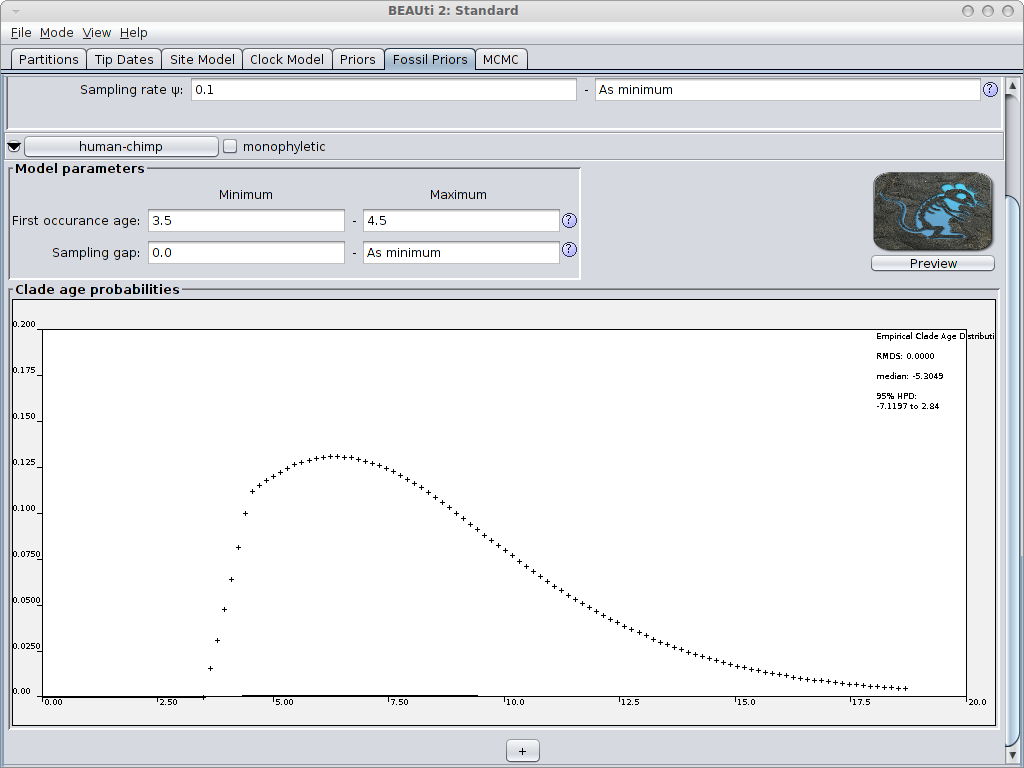
\includegraphics[width=\textwidth,clip=true]{preview.png}\end{center}
After specifying minimum and maximum occurrence age (and optionally the sampling gap),
you can use the 'preview' button to calculate a distribution. The pane at the bottom
shows the shape of the distribution and some statistics such as 95\% highest probability
density interval. Here, we specified a fossil occurrence age range of 3.5 to 4.5 million
year. The distribution shows a slight discontinuity at 4.5 million years as a result.

By using the '+' button, as many fossil calibrations can be specified as you like.
They appear as a list under the common parameters.
\begin{center}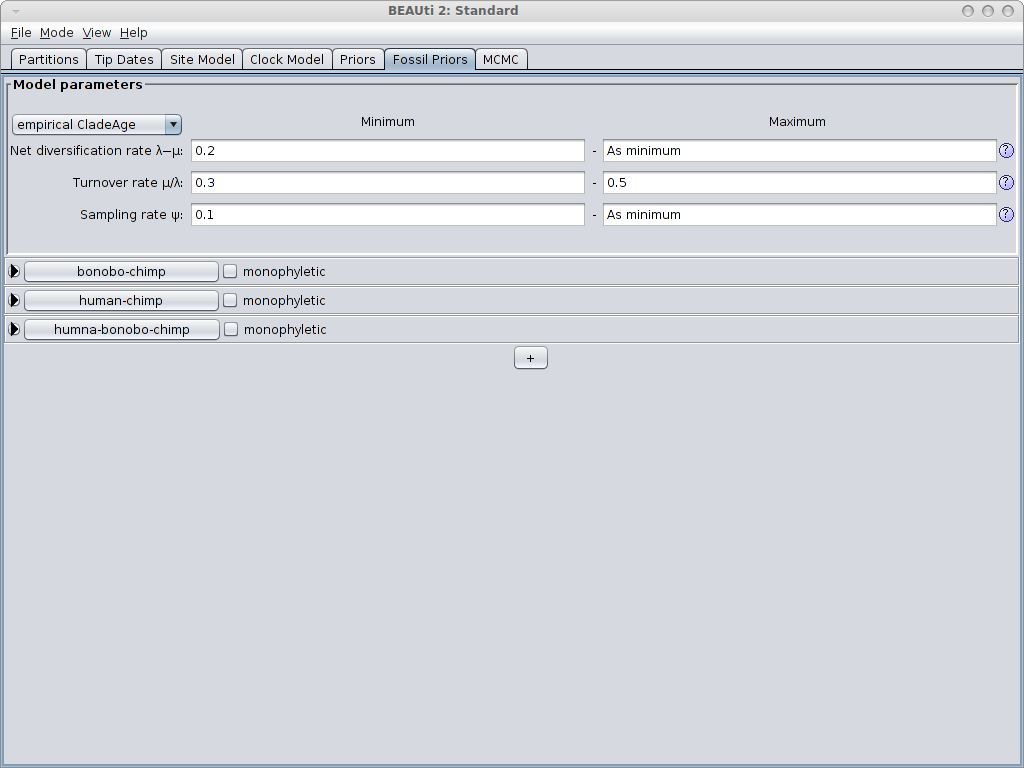
\includegraphics[width=\textwidth,clip=true,trim=0 300 0 0]{fossilPriorsTab3.png}\end{center}

\subsection{Units}
Note that the units used for calibrations should match those used for other
parts of the model, so if you specify fossil calibrations in millions of years, the
clock prior should be in million of years as well. Obviously, the tree is interpreted
in millions of years as well.

\subsection{Which fossils to use}
Obviously, only fossils for which there is morphological evidence that there are
taxa in your alignment should be considered.
If there are multiple fossils for a particular clade, only the oldest should be
used in the analysis.

If there are two fossils for two sister lineages, both fossils should be used, even
though they put a restriction on the same node.

\subsection{Which clades to use}
The fossil calibration applies to the originate of the clade, not the clade itself.
So, the contribution to the posterior comes from the age of the parent clade.
For example, in the following tree we have a fossil associated with a clade
containing a single lineage -- the red dot. The fossil calibration applies to the
parent of the lineage, so a density $f(t_o|\theta)$ (where $\theta$ represent the
fossil calibration parameters, including time of fossil occurrence $t_f$) is contributed 
to the posterior.
\begin{center}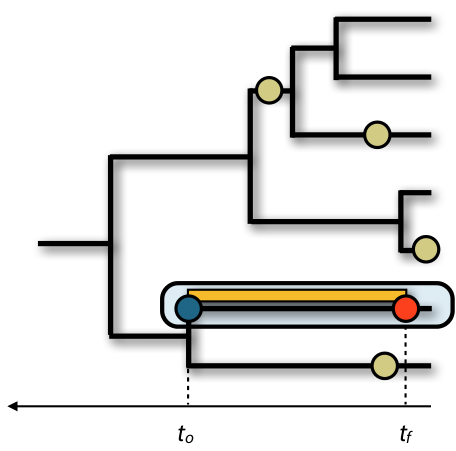
\includegraphics[width=0.5\textwidth,clip=true]{originate.png}\end{center}
One implication is that if you have two fossils from sister lineages, they still
should both be used even though they induce a contributing $f(t_o|\theta_A)f(t_o|\theta_B)$
(where $\theta_A$ and $\theta_B$ the parameters for fossil A and fossil B respectively)
to the posterior from the same node. 
\begin{center}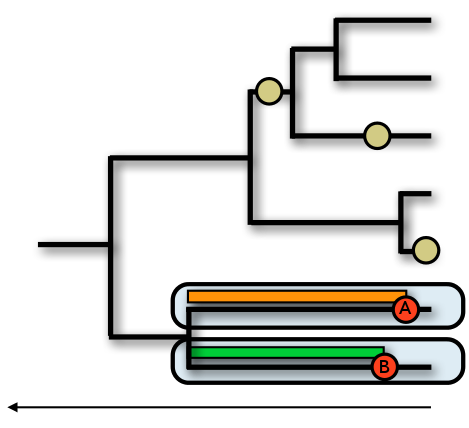
\includegraphics[width=0.5\textwidth,clip=true]{sisterLineages.png}\end{center}

If a fossil is the oldest representative of a smaller clade, but also of a
larger clade, the fossil calibration with the same parameters can be used for 
both the smaller and the larger clade.  For example, in the figure below
Fossil A is used for clade \{1,2,3\}, but also for clade \{1,2,3,4,5\}.
\begin{center}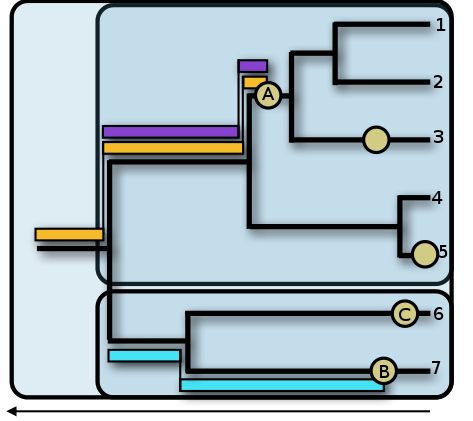
\includegraphics[width=0.5\textwidth,clip=true]{clades.png}\end{center}
Note that if fossil 1 and fossil 2 are on sister lineages, only the oldest of 
the two should be used for the larger clade. In the figure above, fossil B
is older than fossil C, so fossil C should be used for clade \{6\} but
not for clade \{6,7\}. Likewise, fossil B is younger than fossil A, so 
(assuming the image represents a subset of taxa, and there are more outside
this set) fossil A can be used to calibrate \{1,2,3,4,5,6,7\}, but
fossil B should not be used for this clade.




\begin{thebibliography}{99}
\bibitem{AlbaEtAl2001}{Alba DM, Agust\'{i} J, Moy\`{a}-Sol\`{a} S (2001) Completeness of the mammalian fossil record in the Iberian Neogene. Paleobiology 27, 79-83. \url{http://www.jstor.org/stable/2666030}}
\bibitem{AlfaroEtAl2009}{Alfaro ME, Santini F, Brock CD et al. (2009) Nine exceptional radiations plus high turnover explain species diversity in jawed vertebrates. Proceedings of the National Academy of Sciences USA, 106, 13410-13414. \url{http://www.ncbi.nlm.nih.gov/pubmed/19633192}}
\bibitem{Bapst2012}{Bapst DW (2012) paleotree: an R package for paleontological and phylogenetic analyses of evolution. Methods in Ecology and Evolution 3, 803-807 \url{http://onlinelibrary.wiley.com/doi/10.1111/j.2041-210X.2012.00223.x/abstract}}
\bibitem{FooteRaup1996}{Foote M, Raup DM (1996) Fossil preservation and the stratigraphic ranges of taxa. Paleobiology 22, 121-140. \url{http://www.ncbi.nlm.nih.gov/pubmed/11539203}}
\bibitem{Foote1997}{Foote (1997) Estimating taxonomic durations and preservation probability. Paleobiology 23, 278-300. \url{http://www.jstor.org/stable/2401105}}
\bibitem{FooteEtAl1999}{Foote et al. (1999) Evolutionary and preservational constraints on origins of biologic groups: divergence times of eutherian mammals. Science 283, 1310-1314. \url{http://www.ncbi.nlm.nih.gov/pubmed/10037598}}
\bibitem{FooteSepkoski1999}{Foote \& Sepkoski (1999) Absolute measures of the completeness of the fossil record. Nature 398, 415-417. \url{http://www.ncbi.nlm.nih.gov/pubmed/11536900}}
\bibitem{Foote2001}{Foote (2001) Inferring temporal patterns of preservation, origination, and extinction from taxonomic survivorship analysis. Paleobiology 27, 602-630. \url{http://www.jstor.org/stable/1558093}}
\bibitem{FriedmanBrazeau2011}{Friedman \& Brazeau (2011) Sequences, stratigraphy and scenarios: what can we say about the fossil record of the earliest tetrapods? Proc R Soc Lond B, 432-439.  \url{http://www.ncbi.nlm.nih.gov/pubmed/20739322}}
\bibitem{JetzEtAl2012}{Jetz W, Thomas GH, Joy JB, Hartmann K, Mooers A\O  (2012) The global diversity of birds in space and time. Nature, 491, 444-448. \url{http://www.ncbi.nlm.nih.gov/pubmed/23123857}}
\bibitem{PressEtAl1992}{Press WH, Flannery BP, Teukolsky SA, Vetterling WT (1992) Numerical Recipes in Fortran 77: The Art of Scientific Computing. Cambridge University Press. \url{http://apps.nrbook.com/fortran/index.html}}
\bibitem{RaboskyEtAl2013}{Rabosky DL, Santini F, Eastman J, et al. (2013) Rates of speciation and morphological evolution are correlated across the largest vertebrate radiation. Nature Communications 4, 1958. \url{http://www.ncbi.nlm.nih.gov/pubmed/23739623}}
\bibitem{SantiniEtAl2009}{Santini F, Harmon LJ, Carnevale G, Alfaro ME (2009) Did genome duplication drive the origin of teleosts? A comparative study of diversification in ray-finned fishes. BMC Evolutionary Biology, 9, 194. \url{http://www.ncbi.nlm.nih.gov/pubmed/19664233}}
\bibitem{SolowSmith1997}{Solow AR, Smith W (1997) On fossil preservation and the stratigraphic ranges of taxa. Paleobiology 23, 271-277. \url{http://www.jstor.org/stable/2401104}}
\bibitem{Stadler2011}{Stadler T (2011) Mammalian phylogeny reveals recent diversification rate shifts. Proceedings of the National Academy of Sciences, 108, 6187-6192. \url{http://www.ncbi.nlm.nih.gov/pubmed/21444816}}
\end{thebibliography}

\end{document}

